\begin{frame}
    \frametitle{Распространенные форматы данных}
    \begin{itemize}
        \item Стандарт Well-known text (WKT)
        \item shape-файлы ESRI
        \item файлы MapInfo
    \end{itemize}
\end{frame}
\note{
Рассказать о том, что есть форматы данных, которые используются повсеместно по
историческим причинам (Shp, MapInfo). О том как неудобен такой зоопарк. Далее переход
к стандарту WKT.
}


%~ \begin{frame}\label{MapInfoVectorFormat}
    %~ \frametitle{файлы MapInfo}
%~
%~ \end{frame}
%~
%~
%~ \begin{frame}\label{ShpVectorFormat}
    %~ \frametitle{ESRI shp}
%~
%~ \end{frame}


\begin{frame}
    \frametitle{Стандарт WKT: общие сведения}

    \begin{block}{Well-known text}
        WKT --- язык описания векторных геометрических объектов, а так же систем координат пространственных объектов.
    \end{block}

    Существует бинарный формата эквивалент, который называется Well-known binary (WKB), предназначенный для передачи данных
    между различными базами данных.

    Форматы были разработаны OGC (Open Geospatial Consortium).
\end{frame}
\note{
Сказать, что формат нужен, в первую очередь, чтобы посмотреть <<глазами>> на координаты --- текстовый
формат проще для обработки вручную, чем бинарный. Но точно также, как текствый, есть двоичный формат, который
может быть использован и для передачи, и для хранения данных.

Рассказать, где можно посмотреть на примеры использования таких форматов (Postgis, Spatialite) и чем он там удобен.
}

\begin{frame}[fragile]
    \frametitle{WKT: основные элементы}
    \begin{itemize}
        \item POINT: Указываются координаты точки, например, POINT (30 10);
        \item LINESTRING: Указывавается набор координат --- узлов линии, например: LINESTRING (30 10, 10 30, 40 40)
        \item POLYGON: Указывается набор
        координат --- узлов границы
        полигона, например: POLYGON ((30 10, 40 40, 20
        40, 10 20, 30 10)). При этом первая точка
        совпадает с последней. Полигоны могут содержать <<дырки>>, которые указываются после того, как задана
        его граница, например,
        POLYGON ((35 10, 45 45, 15 40, 10 20, 35 10), (20 30, 35 35, 30 20, 20 30))
    \end{itemize}

    Существуют модификации для работы с мультигеометриями: MULTYPOINT, MULTYLINESTRING, MULTYPOLYGON.
\end{frame}
\note{
Описание элементов. Для каких объектов какие элементы используются, примеры.
}

\begin{frame}
    \frametitle{Дополнительные элементы, используемые во внутреннем представлениии}
    Элементы, которые необходимы для ускорения работы с данными:
    \begin{itemize}
        \item Центроид.
        \item Охватывающий прямоугольник.
    \end{itemize}
\end{frame}


\begin{frame}
    \frametitle{Пространственый индекс}
    \begin{figure}[!ht]
        \begin{center}
            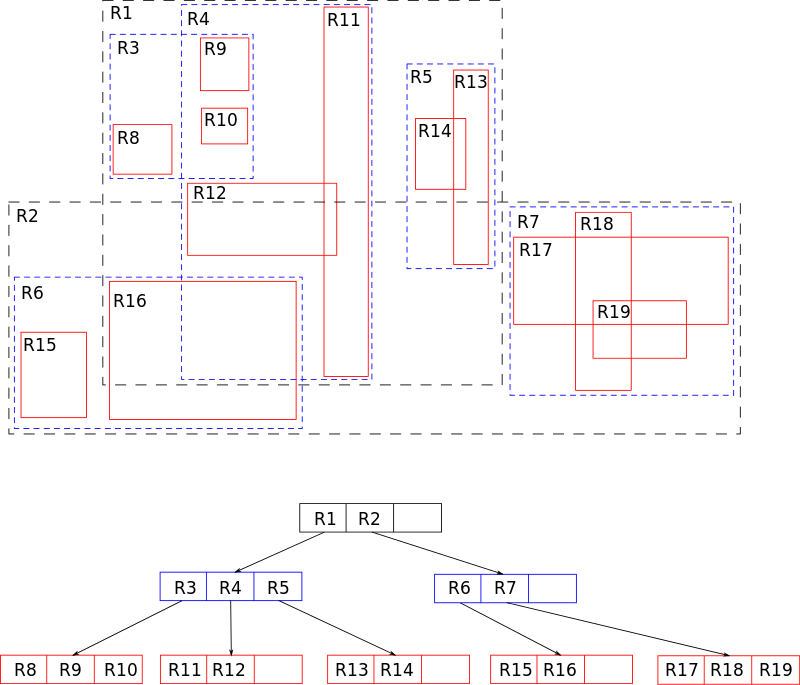
\includegraphics[width=0.8\columnwidth]{./vector_data/img/Rtree}
        \end{center}
    \end{figure}
\end{frame}



